% Format teze zasnovan je na paketu memoir
% http://tug.ctan.org/macros/latex/contrib/memoir/memman.pdf ili
% http://texdoc.net/texmf-dist/doc/latex/memoir/memman.pdf
% 
% Prilikom zadavanja klase memoir, navedenim opcijama se podešava 
% veličina slova (12pt) i jednostrano štampanje (oneside).
% Ove parametre možete menjati samo ako pravite nezvanične verzije
% mastera za privatnu upotrebu (na primer, u b5 varijanti ima smisla 
% smanjiti 

\documentclass[12pt,oneside]{memoir}
\renewcommand{\figurename}{Slika}

% Paket koji definiše sve specifičnosti mastera Matematičkog fakulteta
\usepackage[latinica]{matfmaster}
%
% Podrazumevano pismo je ćirilica.
%   Ako koristite pdflatex, a ne xetex, sav latinički tekst na srpskom jeziku
%   treba biti okružen sa \lat{...} ili \begin{latinica}...\end{latinica}.
%
% Opicija [latinica]:
%   ako želite da pišete latiniciom, dodajte opciju "latinica" tj.
%   prethodni paket uključite pomoću: \usepackage[latinica]{matfmaster}.
%   Ako koristite pdflatex, a ne xetex, sav ćirilički tekst treba biti
%   okružen sa \cir{...} ili \begin{cirilica}...\end{cirilica}.
%
% Opcija [biblatex]:
%   ako želite da koristite reference na više jezika i umesto paketa
%   bibtex da koristite BibLaTeX/Biber, dodajte opciju "biblatex" tj.
%   prethodni paket uključite pomoću: \usepackage[biblatex]{matfmaster}
%
% Opcija [b5paper]:
%   ako želite da napravite verziju teze u manjem (b5) formatu, navedite
%   opciju "b5paper", tj. prethodni paket uključite pomoću: 
%   \usepackage[b5paper]{matfmaster}. Tada ima smisla razmisliti o promeni
%   veličine slova (izmenom opcije 12pt na 11pt u \documentclass{memoir}).
%
% Naravno, opcije je moguće kombinovati.
% Npr. \usepackage[b5paper,biblatex]{matfmaster}

% Ostali paketi koji se koriste u dokumentu
\usepackage{listings} % listing programskog koda
\lstset { %
    language=C++,
    backgroundcolor=\color{black!5}, % set backgroundcolor
    basicstyle=\footnotesize,% basic font setting
}

% Ime kandidata na srpskom jeziku (u odabranom pismu)
\autor{Strahinja Stanojević}
% Naslov teze na srpskom jeziku (u odabranom pismu)
\naslov{Proširivanje alata KLEE naprednim algoritmom pretrage stabla izvršavanja programa}
% Godina u kojoj je teza predana komisiji
\godina{2020}
% Ime i afilijacija mentora (u odabranom pismu)
\mentor{doc. dr Milena Vujošević Janičić, docent\\ Univerzitet u Beogradu, Matematički fakultet}
% Ime i afilijacija prvog člana komisije (u odabranom pismu)
\komisijaA{doc. dr Vesna Marinković, docent\\ Univerzitet u Beogradu, Matematički fakultet}
% Ime i afilijacija drugog člana komisije (u odabranom pismu)
\komisijaB{prof. dr Saša Malkov, vanredni profesor\\ Univerzitet u Beogradu, Matematički fakultet}
% Ime i afilijacija trećeg člana komisije (opciono)
% \komisijaC{}
% Ime i afilijacija četvrtog člana komisije (opciono)
% \komisijaD{}
% Datum odbrane (obrisati ili iskomentarisati narednu liniju ako datum odbrane nije poznat)
\datumodbrane{15. januar 2016.}

% Ključne reči na srpskom jeziku (u odabranom pismu)
\kljucnereci{}

\begin{document}
% ==============================================================================
% Uvodni deo teze
\frontmatter
% ==============================================================================
% Naslovna strana
\naslovna
% Strana sa podacima o mentoru i članovima komisije
\komisija
% Strana sa posvetom (u odabranom pismu)
%\posveta{Мами, тати и деди}
% Strana sa podacima o disertaciji na srpskom jeziku
% \apstrakt
% Sadržaj teze
\tableofcontents*

% ==============================================================================
% Glavni deo teze
\mainmatter
% ==============================================================================

% ------------------------------------------------------------------------------
\chapter{Uvod}
% ------------------------------------------------------------------------------

\section{}

% ------------------------------------------------------------------------------
\chapter{Simboličko izvršavanje} \label{chp:simbolicko_izvrsavanje}
U ovom poglavlju će biti opisani opšti principi na kojima se temelji simboličko izvršavanje u okviru mnogo šire oblasti računarstva, verfikacije softvera. U okviru verifikacije softvera postoje dve velike oblasti, \textit{statička verifikacija softvera} i \textit{dinamička verifikacija softvera}. Statička verifikacija softvera se odnosi na tehnike verifikacije softvera kod kojih je moguće otkrivanje grešaka i rizičnog ponašanja napisanog programskog koda bez njegove prethodne kompilacije i pokretanja. Kod dinamičke verifikacije je nepohodno kompajlirati kod, pokrenuti ga, i tek je onda moguće otkriti greške i kritične delove. Simboličko izvršavanje je jedna od tehnika statičke verifikacije softvera, odnosno bavi se statičkom analizom koda. Jedna je od najkorišćenijih tehnika statičke verifikacije. Na primer, još od 2008. nad većinom Majkrosoftovih (eng. \textit{Microsoft}) aplikacija se vrši 24/7 verifikacija pomoću simboličkog izvršavanja, pre nego što aplikacije budu objavljene. Dodatno, skoro 30\% grešaka u operativnom sistemu Windows 7 je pronađeno baš korišćenjem ove tehnike. Ova činjenica se odnosi na greške koje nisu bile otkrivene korišćenjem drugih tehnika za statičku i dinamičku analizu softvera. 

\section{Osnovni primer simboličkog izvršavanja}
Na početku ovog poglavlja je ukratko opisano šta predstavlja simboličko izvršavanje. U ovom delu će detaljnije biti objašnjeno na koji način simbioličko izvršavanje radi na primeru jedne jednostavne funkcije. 
\newpage
    \begin{lstlisting}[caption={Osnovni primer simboličkog izvršavanja},captionpos=b,label={lst:osnovni_primer}]
        1. void foo(int a, int b) {
        2.   int x = 1, y = 0;
        3.   if (a != 0) {
        4.     y = x + 3;
        5.     if (b == 0)
        6.       x = 2 * (a + b);
        7.   }
        8.   assert(x - y != 0);
        9. }
    \end{lstlisting}

\noindent Razmotrimo primer \ref{lst:osnovni_primer}. Postavlja se pitanje u kojim situacijama može doći do narušavanja ograničenja koje je zadato naredbom $assert()$. 
Konkretno izvršavanje programa radi isključivo sa konkretnim (unapred određenim) vrednostima svih promenljivih. U datom primeru znamo vrednosti za promenljive $x$ i $y$ i one se nazivaju konkretnim promenljivima. Međutim, ukoliko se prethodni k\^od izvršava konkretno, za promenljive $a$ i $b$ je neophodno odrediti vrednosti pre izvršavanja. Ove promenljive se nazivaju \textit{simboličke} i one mogu uzeti bilo koju vrednost iz opsega vrednosti koje mogu biti upisane u promenljivu tipa $int$. Kako promenljive ovog tipa mogu uzeti samo neku od unapred definisanih vrednosti male su šanse da će se konkretnim izvršavanjem, za promenljive kojima nisu dodeljene vrednosti u kodu, generisati baš one vrednosti koje bi dovele do greške. Za razliku od konkretnog izvršavanja, simboličko izvršavanje može odjednom da istražuje veći broj putanja u kodu kroz koje se može proći zavisno od ulaznih podataka (u prethodnom primeru, ulazne vrednosti su vrednosti promenljivih $a$ i $b$). \newline
\indent Osnovna ideja simboličkog izvršavnja je da se vrši simboličko, a ne konkretno izvršavanje. Za svaku od otkrivenih putanja tokom izvršavanja koda se čuvaju sledeći podaci: formula logike prvog reda koja predstavlja uslove koji su bili zadovoljeni u grananjima kroz koja se prošlo i koji su doveli do konkretne putanje i simbolički memorijski prostor u kome se čuvaju vrednosti simboličkih promenljivih. Grananja dovode do ažuriranja formule, dok dodeljivanje vrednosti simboličkim promenljivima dovodi do ažuriranja simboličkog memorijskog prostora. \\
\indent Nakon određivanja neke od putanja vrši se provera zadovoljivosti logičke formule koja odgovara putanji. Za ove potrebe se obično koristi SMT rešavač [?]. SMT rešavač proverava da li pod nekim uslovima (konkretnim vrednostima simboličkih promenljivih) može doći do narušavanja ograničenja koje treba da važi na putanji. Ukoliko postoje takve vrednosti alat za simboličko izvršavanje će dati informaciju pod kojim uslovima može doći do narušavanja zadatih ograničenja.

\begin{figure}[ht]
    \centering
    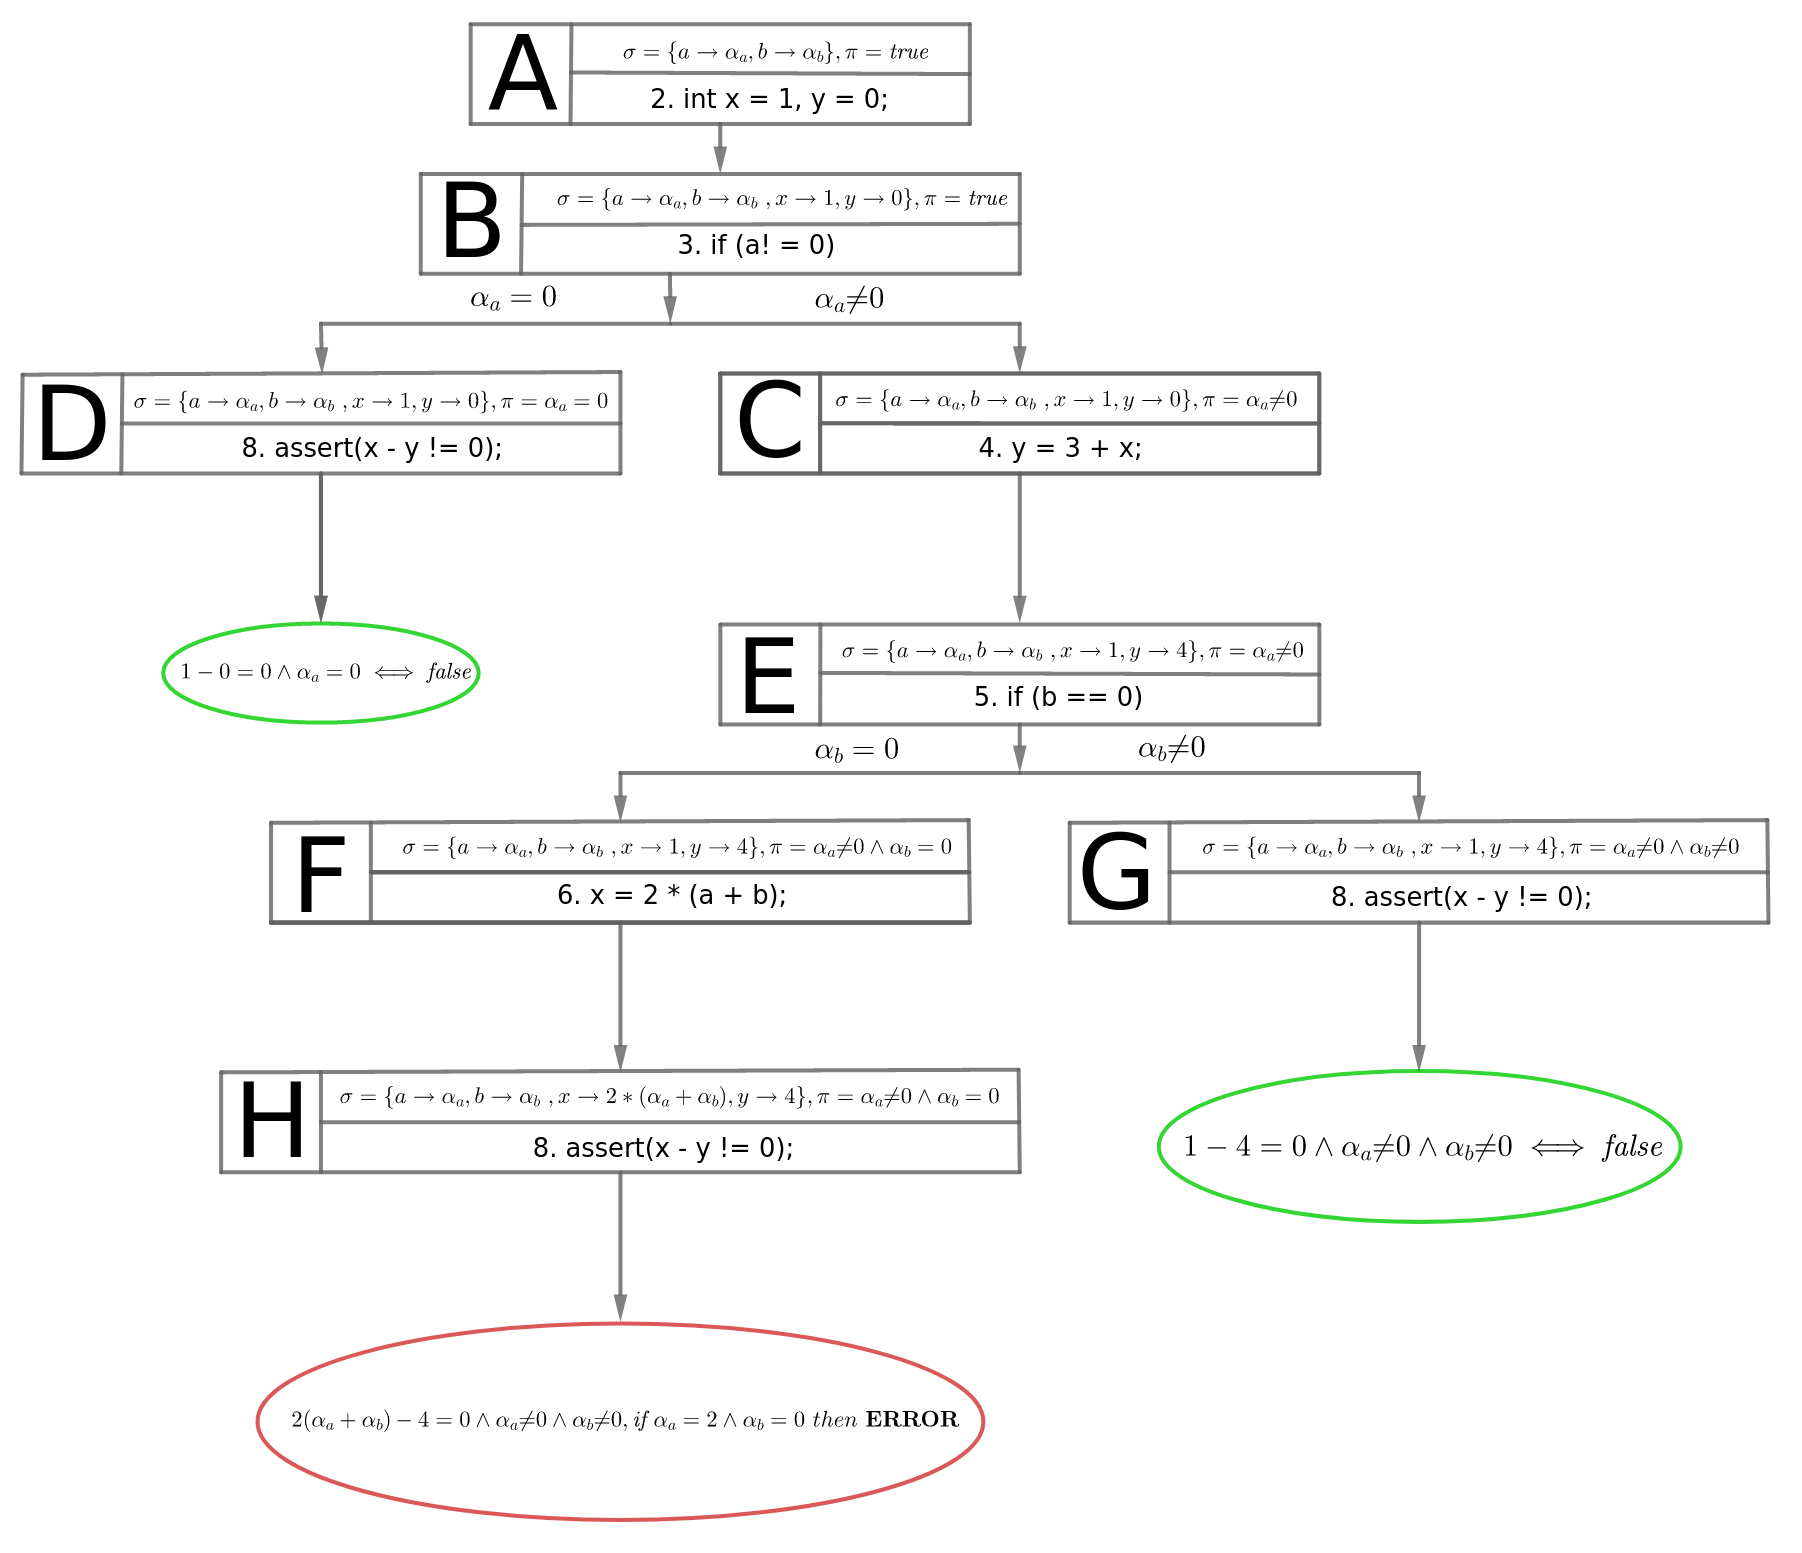
\includegraphics[width=1.0\linewidth]{osnovni_primer.png}
    \caption{Stablo stanja simboličkog izvršavanja koje odgovara primeru. Crvenom elipsom je predstavljeno završno stanje kod koga može doći do greške, dok su zelenim elipsama označena završna stanja kod kojih nema grešaka.}
    \label{fig:osnovni_primer}
\end{figure}

Na slici \ref{fig:osnovni_primer} su prikazana stanja koja odgovaraju simboličkom izvršavanju koda prikazanog u primeru \ref{lst:osnovni_primer}. Sva stanja su oblika $(stmt, \sigma, \pi)$, gde važi sledeće:

\begin{itemize}
    \item $stmt$ je naredba koja se izvršava u datom stanju, odnosno sledeća naredba na koju se naišlo u kodu.
    \newpage
    \item $\sigma$ predstavlja simbolički memorijski prostor u koji se smeštaju vrednosti koje su dodeljene simboličkim promenljivima. Primećujemo da se ove vrednosti dok nisu poznate označavaju sa $\alpha_i$. Iste oznake se koriste i za druge podatke koji nisu unapred poznati (nije ih moguće odrediti statičkom analizom koda) kao što su rezultzati izvršavanja sistemskih poziva, čitanje iz tokova (eng. \textit{streams}) i slično.
    
    \item $\pi$ je formula logike prvog reda koja predstavlja skup uslova koji važe u trenutnom stanju. Ovi uslovi se nadograđuju prolaskom kroz različite naredbe grananja u kodu. Na početku, dok još ne postoji nijedno ograničenje koje treba da važi, odnosno dok se ne naiđe na neko grananje, važi $\pi = true$. 
\end{itemize}

Zavisno do naredbe $stmt$ alat za simboličko izvršavanje radi sledeće:

\begin{itemize}
    \item ako je u pitanju naredba dodele \texttt{x = p} simbolički memorijski prostor $\sigma$ se menja tako što se promenljivoj $x$ u tom prostoru dodeljuje vrednost $p_s$ gde $p_s$ predstavlja vrednost izraza sa desne strane operatora dodele. To može biti konkretna vrednost, ili vrednost nekog kompleksnijeg izraza koja se evaluira u konkretnom stanju zavisno od uslova koji važe. Dodelu označavamo sa $x \rightarrow p_s$.
    
    \item ako je $stmt$ naredba grananja \texttt{if $e$ then $s_{true}$ else $s_{false}$}, ažurira se formula $\pi$. Stanje u kome je došlo do grananja se deli na 2 druga stanja, jedno u kome se dodaje uslov $s_{true}$ i drugo u kome se dodaje uslov $s_{false}$. Formule koje odgovaraju ovim stanjima su $\pi \land e_s$ i $\pi \land \neg e_s$ redom, gde važi da je $e_s$ simbolički izraz koji se dobija evaluacijom izraza $e$.
\end{itemize}

Graf simboličkog izvršavanja može biti predstavljen stablom, što se može primetiti na slici \ref{fig:osnovni_primer}. Incijalno u korenu stabla (stanje $A$) imamo formulu $\pi$ koja ima vrednost \textbf{tačno} (eng. \textit{true}), i promenljivima $a$ i $b$ su dodeljene simboličke vrednosti $\alpha_a$ i $\alpha_b$. Stanje $B$ odogvara prvoj naredbi unutar funkcije $foo$ u kojoj se promenljivima $x$ i $y$ dodeljuju vrednosti 1 i 0 redom, čime one postaju konkretne promenljive. U stanju $B$ se memorijski prostor $\sigma$ ažurira tako što se menjaju vrednosti promenljivih $x$ i $y$. Sledeća naredba je naredba grananja pa se stanje $B$ deli na dva stanja, $C$ i $D$. Stanja $C$ i $D$ odgovaraju uslovima $\alpha_a \neq 0$ i $\alpha_a = 0$ redom, što se može i videti na osnovu ažuriranja formule $\pi$ u odgovarajućim stanjima. Daljom analizom se može zaključiti da su stanja $D$, $G$ i $H$ završna stanja, tj. stanja u kojima se izvršava poslednja naredba funkcije $foo$. Jedina formula koja može dovesti do greške je ona u stanju $H$. Bilo koje ulazne vrednosti za simboličke promenljive $a$ i $b$ za koje važi
\vskip 0.2in
\centerline{$2(\alpha_a + \alpha_b) - 4 = 0 \land \alpha_a \neq 0 \land \alpha_b = 0$}
\vskip 0.2in
\noindent će dovesti do narušavanja uslova naredbe $assert$. Vrednosti koje bi dovele do greške se mogu odrediti pozivanjem $SMT$ rešavača, u datom primeru to su vrednosti $a = 2$ i $b = 0$.
\section{Izazovi simboličkog izvršavanja}

Osnovna ideja simboličkog izvršavanja je da se detaljnom analizom svih putanja kroz koje se može proći u kodu pronađu ulazne vrednosti koje bi mogle dovesti do grešaka. Teorijski gledano ovo je odličan koncept koji garantuje da nema \textit{saglasnost} (eng. \textit{soundness}) i \textit{kompletnost}. Saglasnost garantuje da neće biti lažno pozitivnih rezlutata, tj. da će svi ulazi koji mogu dovesti do grešaka biti otkriveni, dok kompletnost garantuje da neće biti lažno negativnih rezultata, što znači da svi ulazni podaci koji se odrede kao kritični, tj. oni koji mogu dovesti do grešaka, upravo to i jesu. U praksi, vrlo često ovo nije moguće postići jer se obično radi sa velikim softverom, tako da se obično zarad performansi žrtvuje saglasnost. Neki od glavnih izazova sa kojima se suočava simboličko izvršavanje su: 

\begin{itemize}
    \item \textbf{Eksplozija stanja}: na koji način se rešava problem eksplozije stanja? Petlje, rekurzija ili ugnježdene naredbe grananja unutar petlji dovode do ogromnog broja stanja. Nije realno očekivati da alat za simboličko izvršavanje može sve ove putanje da istraži u razumnom vremenu.
    
    \item \textbf{Memorija}: na koji način alati za simboličko izvršavanje rade sa pokazivačima, nizovima, višedimenzionim nizovima, strukturama, klasama i drugim kompleksnim objektima.

    \item \textbf{Rešavanje ograničenja}: SMT rešavaču može biti potrebno mnogo vremena da reši neka kompleksna ograničenja (formule logike prvog reda).
\end{itemize}

\noindent Način rešavanja navedenih problema u alatu KLEE će biti razmotren u poglavlju \ref{KLEE}.

\section{Osnovni principi rada alata za simboličko izvršavanje}
Teorijska ideja simboličkog izvršavanja je da se istraže sve moguće putanje u okviru nekog koda (softvera) i da se odrede sve kombinacije ulaznih podataka koje bi dovele do grešaka. U praksi to nije moguće zbog ranije navedenih problema, pa samim tim alati za simboličko izvršavanje ne pretražuju sve moguće putanje. Jedan od dodatnih problema pored ranije navedenih zbog kog je nemoguće pronaći sve moguće putanje je taj što u realnom softveru postoji k\^od iz eksternih biblioteka kojima sam alat nema pristup, samim tim ne može da generiše sve putanje kroz taj deo koda. Sporedni efekti prilikom izvršavanja koda (kako programski koji se tiču simboličkih promenljivih tako i neki drugi koji se tiču arhitekture računara) mogu predstavljati problem pri rekonstrukciji kompletnog steka softvera koji se analizira. Osnovna ideja za rešavanje ovih problema je kombinovanje konkretnog i simboličkog izvršavanja, takozvano \textit{konkoličko izvršavanje} (eng. \textit{concolic}), što je kovanica reči \textit{concrete} i \textit{symbolic}.
\newline
\newline
\textbf{Dinamičko simboličko izvršavanje}. Jedna od popularnih metoda konkoličnog simboličkog izvršavanje je dinamičko simboličko izvršavanje (eng. \textit{Dynamic Symbolic Execution} ili $DSE$). Ideja iza ovog metoda je da simboličko izvršavanje bude vođeno konkretnim izvršavanjem. Pored simboličkog memorijskog prostora i formula koje predstavljaju ograničenja na različitim putanjama, alat za simboličko izvršavanje čuva i konkretan memorijski prostor $\sigma_c$. Na početku izvršavanja je potrebno odrediti konkretne vrednosti za ulazne podatke, a zatim se sam k\^od izvršava i konkretno i simbolički, paralelno ažurirajući oba memorijska prostora i odgovarajuća ograničenja koja odgovaraju putanjama. Kada se naiđe na naredbu grananja, na osnovu konkretnih vrednosti promenljivih se određuje kojom granom se nastavlja izvršavanje. Granu koja se bira konkretnim izvršavanjem bira i simboličko izvršavanje i na odgovarajući način se ažurira formula $\pi$ koja odgovara putanji. Dakle, simboličko izvršavanje prati konkretno izvršavanje. Ovakav način izvršavanja omogućava da SMT rešavač ne mora da se poziva nakon svakog grananja kako bi se proverilo da li je formula koja se dobija dodavanjem izraza koji odgovara izabranoj putanji nezadovoljiva, jer se to rešava konkretnim izvršavanjem, s obzirom da su konkretne vrednosti promenljivih poznate. Kako bi se istraživale različite putanje, moguće je negirati uslov nekog od grananja i pozvati SMT rešavač kako bi odredio koje su vrednosti ulaznih podataka koje bi dovele do kretanja baš tom putanjom, odnosno koje početne vrednosti ulaznih podataka odgovaraju negiranom uslovu u naredbi grananja. 

Razmotrimo primer \ref{fig:osnovni_primer}. Neka su ulazne vrednosti \texttt{a = 1} i \texttt{b = 1}. Izvršavanje bi krenulo od stanja $A$, 
zatim se prelazi u stanje $B$ gde postoji grananje.
Kako je uslov \texttt{a != 0} ispunjen, izvršavanje bi nastavilo stanjem $C$, nakon čega se nastavlja stanjem $E$ u kome opet imamo grananje. S obzirom uslov $b == 0$ nije ispunjen (jer imamo konkretu vrednost promenljive $b$ koja je $1$, izvršavanje ulazi u završno stanje $G$. 
Konkretan memorijski prostor se kroz ovo izvršavanje menja na sledeći način:
\begin{itemize}
    \item $\sigma_c = {a \rightarrow 1, a \rightarrow 1}$ u stanju $A$,
    
    \item $\sigma_c = {a \rightarrow 1, a \rightarrow 1, x \rightarrow 1, y \rightarrow 4}$ u stanjima $B$ i $C$ i
    
    \item $\sigma_c = {a \rightarrow 1, a \rightarrow 1, x \rightarrow 1, y \rightarrow 0}$ u stanjima $E$ i $G$.
\end{itemize}
U stanju $G$ bi se ustanovilo da je sve u redu, tj. nema narušavanja ograničenja koje je zadato naredbom $assert$, pa se nova putanja može generisati negacijom nekog od uslova koji su bili ispunjeni u naredbama grananja. Recimo da se negira uslov $\alpha_b \neq 0$. SMT rešavač će generisati nove ulazne podatke koji bi zadovoljavali ovaj uslov, recimo \texttt{a = 1\texttt}, \texttt{b = 0} i na taj način bi bila otkrivena nova putanja. U ovom slučaju bi izvršavanje išlo kroz stanja $A \rightarrow B \rightarrow C \rightarrow E \rightarrow F$.

Iako dinamičko simboličko izvršavanje počinje dodelom konkretnih vrednosti promenljivima, nove putanje se generišu negiranjem određenih uslova. Potrebno je odabrati uslov koje naredbe grananja će biti negiran. Broj naredbi grananja (samim tim i broj različitih putanja) u nekom kodu može biti jako veliki, s toga je neophodno na neki način vršiti odabir uslova koji će biti negirani jer je nemoguće u razumnom vremenu proći kroz sve putanje. Načini na koje različiti alati koji vrše dinamičko simboličko izvršavanje biraju koji će uslov biti negiran će biti diskutovan dalje u tekstu. 

U nekim situacijama alat za simboličko izvršavanje koji radi na principu dinamičkog simboličkog izvršavanja ne može da isprati ceo k\^od simbolički. Razlog za to je što se u kodu može desiti da se pozivaju funkcije koje su deo neke eksterne biblioteke čiji izvorni k\^od nije dostupan. \\
Razmotrimo primer \ref{lst:eksterna_1}:
\newpage
\bigbreak
    \begin{lstlisting}[caption={Primer gde rezultat izvršavanja eksterne funkcije nije važan},captionpos=b,label={lst:eksterna_1}]
        void foo(int a, int b)
        {
          int x = bar(a);
          
          if (b > 5)
            ERROR;
        }
    \end{lstlisting}
\bigbreak

Alat bi u ovom slučaju bi promenljivima $a$ i $b$ dodelio neke slučajne vrednosti na početku izvršavanja funkcije $foo$. Pretpostavimo da važi \texttt{a = 1} i \texttt{b = 0}. Sva grananja i sve naredbe koje se izvršavaju u okviru funkcije $bar$ su potpuno nepoznate alatu. Kako bi se otkrila neka nova, potencijalno zanimljiva putanja, potrebno je negirati neki od uslova u grananjima kroz koja se prolazi tokom izvršavanja koda. Jedino grananje koje je poznato je \texttt{if (b > 5)} (izvorni k\^od funckije $bar$ nije dostupan), tako da je moguće negirati uslov baš tog grananja. Na taj način bi se pomoću SMT rešavača dobili novi ulazni podaci za koje mora da važi \texttt{b > 5}, recimo \texttt{a = 1} i \texttt{b = 7}. Na ovaj način bi bila otkrivena nova putanja, i otkrilo bi se da može doći do greške u izvršavanju navedene funkcije.

\bigbreak
    \begin{lstlisting}[caption={Primer gde je rezultat izvršavanja eksterne funkcije važan},captionpos=b,label={lst:eksterna_2}]
        void foo(int a)
        {
          int x = bar(a);
          
          if (x > 0)
            ERROR;
        }
    \end{lstlisting}
\bigbreak

Posmatrajmo sada primer \ref{lst:eksterna_2}. Pretpostavimo da izvorni k\^od funkcije $bar$ nije poznat ni u ovom slučaju. Ono što se može primetiti je da uslov grananja koje je poznato direktno zavisi od rezultata njenog izvršavanja. Recimo da je alat za simboličko izvršavanje generisao ulazne podatke (vrednost za simboličku promenljivu $a$) tako da uslov poznate naredbe grananja nije poznat. SMT rešavač bi pokušao da negira uslov i generiše nove ulazne podatke koji bi trebalo da omoguće otkrivanje nove putanje. Međutim, kako izvorni k\^od funkcije $bar$ nije poznat a uslov grananja direktno zavisi od rezultata njenog izvršavanja nije moguće garantovati da će generisanjem novih ulaznih vrednosti biti otkrivena putanja koja može dovesti do greške. U nekim situacijama je alatu nemoguće da otkrije da ne postoje ulazni podaci koji mogu otkriti novu putanju, tj. da postoji nedostižan kod. Taj slučaj je ilustrovan primerom \ref{lst:eksterna_3}:
    \begin{lstlisting} [caption={Primer u kome može doći do divergencije putanje},captionpos=b,label={lst:eksterna_3}]
        void foo(int a)
        {
          double x = pow(a, 2);
          
          if (x < 0)
            ERROR;
        }
    \end{lstlisting}
\bigbreak

U ovom primeru imamo slučaj gde funkcija $foo$ poziva funkciju $pow$ koja vraća kvadrat svog prvog argumenta argumenta. Neka je alat generisao $a = 5$ kao ulazni podatak. Kako uslov u naredbi grananja nije bio ispunjen, rešavač će otkriti da je potrebno negirati uslov $a \geq 0$. Novi ulazni podatak bi mogao da bude $a = -5$. Međutim, ni na ovaj način se neće desiti da je uslov u naredbi grananja ispunjen. Alat nema mogućnost da otkrije da je nemoguće da dođe do greške, tj. da je naredba u kojoj dolazi do greške nedostižna. \\
Na osnovu prethodnih primera možemo videti da postoje problemi u dinamičkom simboličkom izvršavanju. Neotkrivanje nekih interesantnih putanja, nemogućnost otkrivanja nedostižnog koda. Pozivi eksternih funkcija, kastovanje i simboličkli pokazivači su neki od najvažnijih aspekata o kojima se mora voditi računa prilikom dinamičkog simboličkog izvršavanja kako ne bi došlo do divergencije putanja.\footnote[1]{Divergencija putanja je pojava u dinamičkom simboličkom izvršavanju gde izvršavanje vodi nekom neočekivanom putanjom. Recimo u primeru \ref{lst:eksterna_3} bi bilo očekivano da negacijom uslova grananja bude otkrivena nova putanja, međutim to se nikada neće desiti jer je kvadrat bilo kog broja uvek pozitivan broj.}
\newline
\newline
\textbf{Selektivno simboličko izvršavanje}. Postoji i drugačiji pristup konkoličkom simboličkom  izvršavanju koji vrši alat za selektivno simboličko izvršavanje (eng. \textit{Selective Symbolic Execution} ili $S^2E$). Kod ovog alata simboličko i konkretno izvršavanje se kombinuju na drugačiji način u odnosu na dinamičko simboličko izvršavanje. Neka postoje dve funkcije $A$ i $B$ pri čemu funkcija $A$ poziva funkciju $B$.
Postoje 2 osnovna pristupa:
\begin{enumerate}
    \item \textbf{od konkretnog ka simboličkom i nazad} - funkcija $A$ se izvršava konkretno. Kada se dođe do narebe u kojoj se poziva funkcija $B$, argumenti funkcije se prave simboličkim kako bi se cela funkcija simbolički izvršila i otkrile eventualne greške u istoj. Funkcija $B$ se takođe izvršava i konkretno, a zatim se rezultat konkretnog izvršavanja vraća funkciji $A$ kako bi ona nastavila da se izvršava konkretno.
    
    \item \textbf{od simboličkog ka konkretnom i nazad} - funkcija $A$ se izvršava simbolički. Kada se dođe do narebe u kojoj se poziva funkcija $B$, argumenti funkcije se konkretizuju i funkcija se u potpunosti izvršava konkretno. Nakon izvršavanja funkcije $B$, izvršavanje se vraća na funkciju $A$ koja se nastavlja simbolički.
\end{enumerate}

Ovakav pristup utiče i na saglasnost i na kompletnost rezultata.

\begin{itemize}
    \item \textbf{kompletnost} - potrebno je na neki način izbeći lažno pozitivne rezultate. Kada se funkcija $B$ izvršava simbolički potrebno je voditi računa kroz koje je grane moguće porći zavisno od konkretizacije argumenata, jer izvršavanje funkcije $B$ direktno zavisi od vrednosti promenljivih u funkciji $A$. Kod selektivnog simboličkog izvršavanja se pri kreiranju formule određene putanje u simboličkom izvršavanju ($\pi$) vodi računa o načinu na koji su argumenti konkretizovani, koje vrednosti mogu da uzmu, koji su to sporedni efekti koji mogu da se dese u funkciji $B$ i koja će biti povratna vrednost funkcije za konkretne vrednosti argumenata.
    
    \item \textbf{saglasnost} - takođe može da dođe do lažno negativnih rezultata što je potrebno izbeći. S obzirom da se argumenti funkcije $B$ konkretizuju nakon povratka u funkciju $A$ je moguće da se kroz neka grananja ne prolazi. Kako bi se ovaj problem rešio, funkcija $B$ se konkretno izvršava veći broj puta, pri čemu se za svako od izvršavanja vodi računa kojom putanjom se prošlo kroz funkciju $B$, i nove konkretne ulazne vrednosti parametara se biraju tako da se kroz $B$ u svakom sledećem izvršavanju ide kroz neke nove putanje.
\end{itemize} 
\bigskip
\textbf{Simboličko izvršavanje unazad} - još jedan vid simboličkog izvršavanja je simboličko izvršavanje unazad (eng Symbolic Backward Execution ili $SBE$). Osnovna ideja ovog pristupa je da se krene od neke naredbe u kodu i da se izvršavanje kreće ka ulaznu, tj. početku rada programa. Ova tehnika se obično koristi kada je potrebno odrediti pod kojim uslovima se može doći do neke konkretne naredbe u kodu, i kojom se putanjom do nje stiže. Osnovna mana ovog pristupa je što je neophodno da postoji graf (stablo) izršavanja samog programa, a konstrukcija tog grafa je često izuzetno skupa i komplikovana operacija.

\section{Algoritmi simboličkog izvršavanja}

Postoji veliki broj različitih algoritama i heuristika koje koriste različiti alati za simboličko izvršavanje. U ovom delu će biti dat njihov kratak prikaz.

\bigbreak

\textbf{DFS} - jedan od osnovnih i najpoznatijih algoritama koji se koriste u simboličkom izvršavanju je pretraga grafa u dubinu (eng. \textit{Depth-First Search} ili $DFS$). Kako simboličko izvršavanje koda možemo predstaviti kao stablo stanja kroz koja se prolazi, a s obzirom da je stablo zapravo aciklički graf, možemo koristiti algoritme za pretragu grafova kako bismo birali sledeće stanje koje će biti izvršavano. Algoritam DFS bira putanju kojom krece inicijalno, prilikom prvog grananja, zatim tu putanju istražuje do kraja. Ide maksimalno u dubinu sve dok se ne dođe do kraja putanje ili dok ne bude ispunjen neki drugi uslov zasutavljanja (dubina rekurzije, broj naredbi koje su izvršene na putanji, vreme koje je provedeno istražujući odrešenu putanju itd). Nakon toga algoritam vrši odsecanje te putanje, vraća se unazad do nekog prethodnog grananja i nastavlja drugim putem. Zatim se ta nova putanja istražuje maksimalno (do kraja, ili nekog drugog uslova izlaska). Algoritam pretrage grafa u dubinu se obično koristi kada je memorija kojom se raspolaže ogranična (ne dovoljno velika za čuvanje velikog broja stanja). Najveća mana ovog pristupa je što jako dugo radi (vrlo često ne može da završi u razumnom vremenu) kada u kodu postoji rekurzivna funkcija koja se izvršava ili ukoliko postoje petlje čije ograničenje nisu konkretne vrednosti već simboličke promenljive. 

\bigbreak

\textbf{BFS} - još jedan često korišćeni grafovski algoritam za pretragu stabla stanja u simboličkom izvršavanju je pretraga grafa u širinu (eng. \textit{Breadth-First Search} ili $BFS$). Pretraga u širinu ima prednosti u odnosu na pretragu u dubinu jer paralelno izučava veliki broj putanja. Na ovaj način se mogu otkriti neka zanimljiva opažanja ranije u odnosu na pretragu u dubinu i češće se koristi ukoliko je vreme ograničeno (previše kratko da bi se čekalo da DFS pretraga istraži jednu po jednu putanju do kraja). Mana ovog algoritma je to što čuva ogroman broj stanja i puni memoriju koja je dodeljena alatu za simboličko izvršavanje. Pošto se veliki broj putanja paralelno izučava potrebno je za sve njih čuvati stanja, formule logike prvog reda čija se zadovoljivost proverava SMT rešavačem (ograničenja koja važe za svaku od putanja), održavati simbolički memorijski prostor i slično. Iz navedenih razloga je potrošnja memorije znatno veća u odnosu na algoritam pretrage u dubinu. Još jedna mana ovog pristupa je što nije realno očekivati da sve putanje mogu biti izučene do kraja. Vreme je često ograničavajući faktor kada govorimo o analizi realnog softvera gde postoji jako veliki broj linija koda pa u tim situacijama algoritam pretrage u širinu ne uspeva da izuči sve putanje do kraja. Međutim, činjenica je da paralelnim izučavanjem većeg broja putanja lakše i brže dolazi do interesantnih zapažanja u odnosu na pretragu u dubinu.

\bigbreak

\textbf{Slučajan odabir narednog stanja} - strategija kod koje se naredno stanje koje će biti obrađeno bira na potpuno slučajan način. Od svih trenutno dostupnih stanja u stablu pretarge na slučajan način se bira jedno od njih. Ova ideja je sama po sebi jako loša jer nema konkretne strategije po kojoj bira sledeće stanje, međutim često se obogaćuje dodatno različitim heuristikama. Neke od heuristika su:

\begin{itemize}
    \item \textbf{Izvršavanje vođeno pokrivenošću koda} - osnovna ideja ove heuristike je da se za svaku putanju određuje njena važnost na osnovu toga koliko instrukcija je u određenoj putanji izvršeno od otkrivanja poslednje nove instrukcije, koliko je udaljena naredna neposećena instrukcija i slično.
    
    \item \textbf{Izvršavanje vođeno podputanjama} - ideja je birati ono stanje koje vodi podputanjom koja je bila izvršena manji broj puta do tog trenutka. Podputanja se definiše kao $n$ uzasptonih naredbi u okviru jedne putanje. Kod ove heuristike ključnu ulogu igra odabir vrednosti $n$. Do sada nije pronađena optimalna vrednost parametra $n$ koja je univerzalna.
    
    \item \textbf{Najkraće simboličko izvršavanje} - ova heurstika se obično koristi kada je potrebno doći do određene instrukcije u samom kodu. Uvek se bira ono stanje koje je najbliže traženoj naredbi. Malo podseća na pretragu vođenu pokrivenošću koda, međutim razlika je u tome da u ovoj strategiji težimo jednoj konkretnoj naredbi, a ne pokrivenošću celokupnog koda.
    
    \item \textbf{Iscrpljivanje petji} - osnovna ideja ove heuristike je da se biraju putanje koje sadrže petlje. Opravdanje je se krije u opažanju da u praksi veliki broj grešaka u radu sa petljama vodi ka prekoračenju bafera\footnote[2]{Divergencija putanja je pojava u dinamičkom simboličkom izvršavanju gde izvršavanje vodi nekom neočekivanom putanjom. Recimo u primeru 3 bi bilo očekivano da negacijom uslova grananja bude otkrivena nova putanja, međutim to se nikada neće desiti jer je kvadrat bilo kog broja uvek pozitivan broj.} i drugim memorijskim problemima.
    
    \newpage
    \item \textbf{Prvo putanje sa greškama} - kod ove heuristike se prvo izučavaju one putanje kod kojih su u nekim ranijim delovima pronađene sitne greške (eng. \textit{bugs}). Intuicija iza ovog pristupa je da ako je putanja u ranijem delu imala neku grešku nije dovoljno dobro istestirana.
\end{itemize}

\textbf{Generacijska pretraga} - ova tehnika uglavnom predstavlja kombinaciju pretrage u dubinu i pretrage vođene pokrivenošću koda. Osnovna ideja je da se pretraga vrši po generacijama. Kreće se od nulte generacije u kojoj se slučajno odabrana putanja izvršava do kraja pomoću algoritma pretrage grafa stanja u dubinu. U prvoj generaciji se iz putanje nulte generacije istražuju nove putanje i to tako što se odredi jedan od uslova grananja u putanji nulte generacije i njegovim negiranjem se dobija sledeća putanja. U $N$-toj generaciji se iz svih putanja prethodne generacije bira uslov koji se negira i pomoću koga se kreće u istraživanje nove putanje. Biranje putanje kojom će se krenuti se vrši heuristikom vođenom pokrivenošću koda.
\bigskip

\textbf{Hibridne strategije} - uglavnom se svode na kombinaciju većeg broja algoritama koji se na određene načine smenjuju prilikom pretrage. Zavisno od specifičnih potreba (otkrivanje putanje do određene naredbe, otkrivanje što većeg broja putanja, pokrivenost koda itd.) koriste se kombinacije različitih algoritama koji se pri izvršavanju smenjuju i kombinuju na različite načine.

\section{Pregled alata za simboličko izvršavanje} \label{alati_za_simbolicko}

Postoji veliki broj različitih alata za simboličko izvršavanje. Većina ovih alata počiva na istim principima:

\begin{itemize}
    \item \textbf{Napredak} - izvršavanje bi trebalo da može da traje neko određeno vreme bez potrošnje svih resursa koji su mu dodeljeni. Tu se pre svega misli na memoriju koja često može biti resurs koji biva brzo iskorišćen u potpunosti zbog velikog broja raličitih putanja i stanja.
    
    \item \textbf{Ponovljen posao} - ne bi trebalo da se neki posao ponavlja. Odnosno, nije dobro da se izvršavanje kreće pokreće od samog početka da bi se otkrile neke nove putanje ako već postoji zajednički prefiks te putanje sa nekim postojećim.
    
    \item \textbf{Analiza i ponovno korišćenje već odrađenog posla} - rezultati prethodnih izračunavanja i saznanja iz prethodnih putanja bi trebalo da se koriste u što većoj meri kako bi se uštedelo vreme, i smanjilo ponavljanje posla što se poklapa sa prethodnom stavkom. Tu se pre svega misli na skupe pozive SMT rešavaču za formule za koje je zadovoljivost proverena ranije. Takve pozive treba izbegavati.
\end{itemize}
\bigskip
Na osnovu toga da li pokušavaju da obrade veći broj putanja odjednom ili jednu po jednu alati za simboličko izvršavanje se mogu podeliti u dve grupe:
\begin{itemize}
    \item \textbf{\textit{online} alati} - alati koji pokušavaju da izvršavaju i izučavaju veći broj putanja odjednom. Kada god se naiđe na grananje vrši se kloniranje trenutnog stanja. Dobra strana ovih alata je što nema ponavljanja posla jer se jednom izvršena instrukcija nikada ne izvršava ponovo. Loša strana je to što veoma brzo pune memoriju koja im je dodeljena, jer moraju da održavaju veliki broj putanja i stanja. Primeri ovakvih alata su KLEE[?], AEG[?], S$^2$E[?].
    
    \item \textbf{\textit{offline} alati} - za razliku od \textit{online} alata, \textit{offline} alati izvršavaju jednu po jednu putanju. Primer ovakvog alata bi bio SAGE[?]. Ideja je izvršiti celu jednu putanju do samog kraja, a zatim preći na neku drugu. Dobra strana ovog pristupa je jako malo korišćenje memorije jer se čuvaju stanja vezana za samo jednu putanju, ali je problem što obično ima mnogo ponavljanja posla. Pretraga nove putanje uglavnom kreće od samog početka. Opšti princip rada \textit{offline} alata je da kreću sa konkretnim izvršavanjem, što znači da je potrebno generisati ulazne podatke. Pamti se put kojim se prošlo pri konkretnom izvršavanju, a zatim se isti put prolazi simbolički. 
    
    \item \textbf{\textit{hibridni} alati} - hibridni alati kao što je Mayhem[?] pokušavaju da pronađu balans između prevelikog utroška memorije i vremena koje je potrebno za izvršavanje. Na početku počinju kao \textit{online} rešavači, a kada se memorija popuni do određene količine prelaze u \textit{offline} izvršavanje.
\end{itemize}
\bigskip
\textbf{DART} - (eng. \textit{Directed Automated Random Testing}) je alat koji vrši konkoličko simboličko izvršavanje i to dinamičko simboličko izvršavanje. Za odabir uslova grananja koji će biti negiran kako bi se otkrila nova putanja se koristi algoritam pretrage u dubinu (DFS). DART je alat koji počiva na 3 osnovna principa:
\begin{enumerate}
    \item\textit{Automatski} izdvaja interfejs programa statičkom analizom izvornog koda.
    
    \item\textit{Slučajno} (eng. \textit{Random}) generiše testove za izdvojeni interfejs programa kako bi se simuliralo što opštije okruženje rada programa.
    
    \item Dinamička analiza ponašanja programa prilikom slučajnog testiranja (prethodna stavka) i automatsko generisanje novih test primera koji \textit{usemravaju} (eng. \textit{Direct}) izvršavanje ka drugim mogućim putanjama.
\end{enumerate}

\noindent DART se uglavnom koristi za testiranje programa napisanih u programskom jeziku \textit{C}. \\
\\
\textbf{SAGE} - još jedan alat koji vrši dinamičko simboličko izvršavanje. Za razliku od DART$-$a, SAGE koristi generacijsku pretragu. Osnovna ideja ovog alata je da sistematski, ali ipak delimično istraži prostor mogućih stanja softvera pri čemu se izbegava ponavljanje posla, a ujedno maksimizuje broj generisanih različitih testova. Pošto se izučava samo deo prostora stanja, ključan je izbor ulaznih vrednosti simboličkih promenljivih. Važnost inicijalnih vrednosti podseća na važnost istih kod tradicionalnog nejasnog testiranja metodom crne kutije (eng. \textit{black-box fuzzy testing}), pa se stoga alati poput SAGE$-$a često nazivaju nejasnim testerima metodom bele kutije (eng. \textit{white-box fuzzy testers}). SAGE je primer \textit{offline} alata. \\
\\
\textbf{S$^2$E} - još jedan poznat alat za simboličko izvršavanje je ranije pomenuti alat S$^2$E koji vrši selektivno simboličko izvršavanje. Jedan je od glavnih predstavnika \textit{online} alata. Pored ranije navedenih osobina treba napomenuti da se za izbor narednog stanja koje se izvršava, samim tim i izbor putanje koja se izučava, vrši heuristikom vođenom pokrivenošću koda. \\
\\
\textbf{Mayhem} - primer \textit{hibridnog} alata za simboličko izvršavanje. Ovaj alat kombinuje tehnike \textit{online} i \textit{offline} alata i to tako što koristi prednosti svake od tehnika. Ova jalat radi direktno sa izvršnim kodom. Kako bi ovo bilo moguće postoje dve važne stavke o kojima Mayhem mora da vodi računa:
\begin{itemize}
    \item Održavanje putanja koje se izučavaju bez potpune potrošnje dostupne memorije.
    
    \item Oprez pri radu sa simboličkom memorijom, odnosno sa simboličkim adresama kako ne bi dolazilo do prekoračenja bafera i sličnih problema.
\end{itemize} 
\medskip
Pored koncepta hibridnog alata, Mayhem još uvodi i memoriju zasnovanu na indeksima, tehniku koja ovom alatu omogućava da efikasno radi sa simboličkom memorijom na binarnom nivou (rad sa izvršnim fajlovima).\\
\\
\textbf{AEG} - \textbf{Automatic Exploit Generation} je alat koji je napravljen kao nadgradnja drugog alata za simboličko izvršavanje, \textit{KLEE-a}. Osnovna ideja ovog alata je da se ne istražuju sve moguće putanje u programu, već da fokus bude na onim putanjama za koje se veruje da imaju veću verovatnoću izvršavanja zavisno od vrednosti ulaznih podataka. Osnovna tehnika kojom se služi ovaj alat je preduslovno simboličko izvršavanje (eng. \textit{preconditioned symbolic execution}). Jedan zasad poznati problem ovog alata je skalabilnost na velikim programima, ali se na tome aktivno radi.
\newpage

\chapter{Alat za simboličko izvršavanje KLEE} \label{KLEE}
\textbf{KLEE} je alat otvorenog koda koji je nastao na Univerzitetu Ilinois. U pitanju je potpuno simbolički alat što znači da su sve promenljive simboličke i nema konkoličkog simboličkog izvršavanja. Ideja alata je da pokuša kompletne programe da izvršava simbolički uz dodatak konkretnih vrednosti koje se u kodu javljaju kao konstante. Dakle, ne generiše se slučajan ulaz i na taj način se prati kojim se putem prolazi zavisno od vrednosti već pokušava da ide različitim putevima odjednom menjajući uslove koji važe. Na primer ako imamo uslov grananja da je $x > 3$ onda KLEE putanju deli na dve disjunktne putanje. U jednoj će važiti $\pi \land x > 3$ a u drugoj negacija tog uslova, odnosno $\pi \land x \leq 3$. Na ovaj način KLEE prolazi kroz obe putanje. Odlika ovog alata je i ta da sve putanje obilazi paralelno, tj. ne izučava jednu putanju do kraja. Stanja koja su vezana za svaku od aktivnih putanja se čuvaju sve vreme bez obzira na algoritam koji se koristi. Razlog za ovako nešto leži u činjenici da je KLEE jedan od \textit{online} alata za simboličko izvršavanje.

\section{Memorijski model}
KLEE čuva vrednosti različitih promenljivih u skladištima. Postoje dva skladišta u okviru alata. 
\begin{itemize}
    \item \textbf{konkretno} - skladište u okviru kog se čuvaju vrednosti konkretnih promenljivih. To su konstante ili promenljive kojima je dodeljena vrednost u kodu. Recimo $int x = 5;$ predstavlja konkretnu promenljivu. Nije potrebno simbolički pratiti koju potencijalnu vrednost ova promenljiva ima. Ona je unapred poznata. Ukoliko se desi da se konkretna promenljiva koristi u nekoj operaciji sa simboličkom ona takođe postaje simbolička, jer zavisno od uslova koji važe za simboličku promenljivu i konkretna menja svoju vrednost u određenoj putanji.
    
    \item \textbf{simboličko} - skladište gde se čuvaju simboličke promenljive. Kako one nemaju konkretne vrednosti sve do trenutka kada se dođe u završno stanje, veći deo vremena se čuva samo njihova adresa. Kada se dođe u završno stanje, potrebno je generisati konkretne vrednosti simboličkih promenljivih na osnovu uslova koji važe u tom stanju. U tom trenutku one dobijaju konkretne vrednosti, i generiše se test primer koji govori o tome koje su vrednosti promenljivih kada se program izvrši kretanjem kroz određenu putanju. Te vrednosti ne moraju biti jednistvene, npr ako u stanju važi uslov $x > 5$ promenljiva $x$ može uzeti bilo koju vrednost koja je veća od $5$. Ukoliko u nekom stanju dolazi do greške pod uslovom $x = 7$ onda će vrednost promenljive $x$ koja se generiše u tom stanju biti baš $7$.
\end{itemize}
\bigskip
Količina radne memorije koja se dodeljuje samom alatu je ograničena i zadaje se kao jedan od parametara prilikom pokretanja samog KLEE-a. Zbog osobine alata da čuva sva stanja koja su vezana za sve putanje koje se izučavaju vrlo često dolazi do situacije gde se memorija popuni. Kada se ovo desi na neki način mora da dođe do ''pražnjenja''. To se radi tako što se odbacuju neka stanja. Broj stanja koja se izbacuju se određuje slučajnom metodom. Generiše se pseudo-slučajan broj i on predstavlja broj stanja koja se izbacuju. Postavlja se pitanje na koji način se biraju stanja koja bivaju izbačena. Ovo se takođe radi slučajno uz još jedan dodatan uslov, a to je da se ne izbacuju stanja koja su otkrila novu instrukciju. Generiše se pseudo-slučajan broj koji govori o indeksu stanja u nizu koje treba da bude izbačeno i ako u njemu nije otkrivena nova instrukcija ono može biti izbačeno. U suprotnom se generiše nov indeks i bira se drugo stanje za izbacivanje iz skupa aktivnih stanja.

\section{Kontrola toka u alatu KLEE}
Rad sa funkcijama u alatu KLEE se ne razlikuje previše od standardnog rada sa funkcijama u nekom programskom jeziku. Neka je potrebno simbolički izvršiti funkciju $f$. I neka to bude funkcija koja se poziva iz funkcije $g$ sa parametrom $a$ bez povratne vrednosti. Dakle, \texttt{void f(int a)}. Postoji ''stek'' na kome se čuvaju lokalne promenljive i parametri funkcije $f$. Takođe se pamti koja je funkcija pozivalac kao i koju naredbu funkcije $g$ treba izvršiti nakon što $f$ bude izvršena. Sve promenljive se i dalje čuvaju u ranije opisanim skladištima. Nakon što se završi izvršavanje funkcije memorija na kojoj su se nalazile lokalne promenljive postaje ''slobodna'', odnosno tu je moguće smeštait nove promenljive neke nove funkcije. Sve rečeno se odnosi samo na funkcije za koje je izvorni k\^od poznat i napisan u programskim jezicima C i C++. Ono što se može desiti je da izvorni k\^od neke funkcije nije poznat uopšte, ili da je napisan u drugom programskom jeziku. Ukoliko se nešto ovako desi KLEE nije u mogućnosti da prati izvršavanje funkcije simbolički. U tim situacijama se argumenti konkretizuju na osnovu uslova koji važe na putanji gde se nalazi poziv funkcije i funkcije se jednostavno poziva i čuva se povratna vrednost ukoliko postoji. Ukoliko je funkcija bez povratne vrednosti pozvana samo se izvršava bez simboličkog praćenja i izvršavanje se nastavlja simbolički u okviru funkcije pozivaoca. 
\indent Kada je reč o petljama KLEE ima prilično specifičan način rada. Naime, kako je alat potpuno simbolički, sve petlje se izvršavaju do kraja kroz sve potencijalne iteracije. Ako važi da je uslov izlaska iz petlje \texttt{i < n} gde je $n$ simbolička promenljiva, KLEE će pokušavati da prođe sve moguće iteracije. Ukoliko bi se znalo da je vrednost promenljive $n$ na primer $1000$ onda bi se petlja vrtela simbolički do vrednosti 1000. Međutim, kada je granica broja iteracija petlje simbolička promenljiva KLEE nema mogućnost da izvrti određen broj iteracija i vidi ponašanje programa, već se ide do maksimalne vrednosti koju može da čuva promenljiva tipa koji odgovara tipu promenljive $n$. Iz ovog razloga KLEE ima veliki problem sa petljama bez obzira na to koji se algoritam koristi. Često u okviru petlji postoje grananja što dovodi do toga da se kreira veliki broj novih stanja u okviru istih. Na ovaj način se i memorija brže puni što dovodi do potrebe za ranije opisanim odbacivanjem nekih stanja. Kada se govori o rekurzivnim funkcijama situacija je veoma slična. Rekurzija se ''vrti'' do uslova izlaska. Ukoliko uislov izlaska iz rekurzije zavisi od simboličke promenljive javlja se isti problem kao i pri radu sa petljama u okviru alata KLEE.

\section{Rad sa pokazivačima i nizovima}
Rad sa pokazivačima se takođe ne razlikuje previše od onoga na šta smo navikli u programskom jeziku C. Postoji poseban deo memorije koji se zove \textit{Known Symbolics} gde se smeštaju promenljive poslate preko pokazivača. Kada je promenljiva prosleđena preko pokazivača funkciji nju je moguće menjati u okviru iste. Ako je u pitanju simbolička promenljiva potrebno je znati koja simbolička promenljiva se ''menja'', tj. koji dodatni uslovi za istu treba da važe. Zato postoji pomenuti deo simboličkog skladišta koji čuva sve simboličke promenljive koje su uvedene do tad. Objekat okazivačke promenljive koja se kreira prilikom poziva funkcije kao jedno od polja čuva i adresu promenljive na koju ''pokazuje''. Na taj način je moguće u okviru dela \textit{Known Symbolics} moguće menjati promenljivu, odnosno uslove koji važe za nju. Ukoliko je promenljiva koja se šalje preko pokazivača konkretna, onda se ''prati'' adresa u okviru konkretnog skladišta i vrednost konkretne promenljive se menja.
Rad sa nizovima dosta podseća na rad sa pokazivačima. Suština obe tehnike je ista. Postoji deo memorije gde se čuvaju simbolički nizovi. Kada se javi potreba za pristupom nekom elementu niza na osnovu indeksa, kao i kod programskog jezika C se to radi tako što se u odnosu na početak niza vrši pomeranje za određeni broj, tj. baš traženi indeks. Zavisno da li se radi o konkretnom ili simboličkom nizu, sve promenljive koje pripadaju istom se čuvaju u odgovarajućem skladištu (konkretnom odnosno simboličkom). Nakon što se javi potreba za pristupom $i$-tom elementu niza, određuje se njegova adresa, tj. kreira se pokazivač na taj element kako bi mu se pristupilo i kako bi eventualno mogao da bude izmenjen. Kao i kod pokazivačkih promenljivih (nizovi u suštini i jesu pokazivači) i kod nizova se elementi konkretnih nizova menjaju u konkretnom skladištu, a elementima simboličkih nizova se dodatna ograničenja dodaju u okviru \textit{Known Symbolics} dela simboličkog skladišta.  

\section{Algoritmi pretrage stabla stanja}
KLEE kao i većina drugih alata u okviru svoje implementacije sadrži vreći broj algoritama za pretragu grafa (stabla) stanja simboličkog izvršavanja. Alat se svrstava u grupu \textit{online} alata što znači da bez obzira na to koji se konkretan algoritam koristi za analizu nekog koda, sve putanje i sva stanja koja su vezana za njih će biti čuvani tokom izvršavanja (dok se putanja ne završi čime se brišu sva stanja vezana za nju pa i ona sama).\newline
\\
\textbf{DFS} je jedan od osnovnih algoritama pretrage grafa stanja u alatu KLEE. U pitanju je klasična pretraga grafa u dubinu. Ideja je istražiti jednu putanju do njenog samog kraja (završnog stanja ili dok se ne ispuni neki drugi uslov prekida istraživanja putanje), a zatim se vrši povratak na neko prethodno grananje gde se ide suprotnim putem od izabranog prilikom tog grananja (slično kao kod pretrage bilo kog grafa u dubinu). Ukoliko imamo stanje A u kome se vrši naredba grananja, u narednom koraku je potrebno da postoje dva stanja (B i C), jer postoji grananje koje može da odvede izvršavanje na dva različita puta. Interna implementacija algoritma pretrage u dubinu u okviru alata KLEE koristi \textit{std::vector<>} pokazivača na stanja izvršavanja (ExecutionState). Svaki put kada se naidje na grananje u stanju A vrši se dodavanje stanja C na kraj vektora, ali se stanje B ne kreira eksplicitno. Umesto toga KLEE vrši ''evoluciju'' stanja A. Ovom stanju se samo dodaju dodatna ograničenja koja treba važe u stanju B, menja se \textit{trenutna} naredba koja se izvršava u stanju da odgovara naredbi koja je trenutna u stanju B i menja se \textit{sledeća} naredba koja takođe odgovara novonastalom stanju. Dakle, jedno stanje evoluira i jedno stanje se dodaje dodaje na kraj vektora stanja svaki put kada imamo naredbu grananja. Kako bi se nad ovakvim grafom (na početku nemamo sve čvorove grafa, već se on formira dinamički) simulirala pretraga u dubinu uvek se za naredno stanje bira poslednje stanje iz vektora. Kasnije u tekstu će biti prikazan primer izvršavanja algoritma DFS gde će se videti kako se vrši simulacija navedenog algoritma. Ukoliko u nekom stanju nema naredbe grananja, vrši se samo ''evolucija'' stanja, tj. dodaju se nova ograničenja, menja se \textit{trenutna} i \textit{sledeća} naredba tog stanja i izvršavanje se nastavlja. Ovo stanje ne menja svoju poziciju u vektoru, već ostaje poslednje. Kada se dođe do završnog stanja ono se samo uklanja iz vektora stanja i uzima se poslednje stanje koje ostaje u vektoru kao naredno čime se nastavlja pretraga stabla u dubinu. Treba obratiti pažnju da iako je uobičajena implementacija DFS algoritma rekurzivna, u implementaciji u alatu KLEE nema rekurzije niti steka kojim bi se simulirala ista, već se algoritam simulira pomoću vektora na već opisani način.\newline
\\
\textbf{BFS} je još jedan osnovni algoritam kako pretrage grafova (samim tim i stabala), tako i pretrage stabla stanja u alatima za simboličko izvršavanje. Za razliku od pretrage grafa u dubinu, ideja pretrage u širinu je, baš kao i kod svakog grafa, da se što veći broj putanja izučava odjednom, odnosno da se izvršavaju sva stanja koja su na jednom nivou stabla, a nakon što se sva stanja sa nekog nivoa izvrše prelazi se na naredni nivo. Ovaj pristup ima prednost u odnosu na prethodni jer ima potencijala da otkrije veći broj zanimljivih stanja i pojava u kodu u ranim fazama putanja. Zamislimo recimo da imamo potpuno binarno stablo.\footnote[3]{Svi čvorovi osim listova imaju tačno dva potomka}. Neka se izvršavanje nalazi na nivou dva gde imamo osam čvorova (stanja). Dodatno, neka je memorija ograničavajući faktor u toj meri da neka stanja moraju biti odbačena jer je nema dovoljno da se izvrši sve do kraja. Zamislimo da na narednom nivou nakon grananja prvog stanja (krajnji levi čvor na nivou) može doći do greške u ''evoluiranom'' stanju. DFS neće biti u stanju da pronađe ovu grešku jer će birati uvek poslednje stanje i kretaće se njime do samog kraja. S druge strane, BFS algoritam će izvršti svih osam stanja drugog nivoa i nakon toga će biti u stanju da već kod narednog stanja (''evoluiranog'') pronađe grešku. U alatu KLEE interna implementacija algoritma pretrage u širniu koristi \textit{std::deque<>} pokazivača na stanja koja se izvršavaju (ExecutionState), kako bi operacije skidanja sa početka i dodavanja na kraj bile efikasne. Slično kao kod algoritma DFS, i BFS samo vrši ''evoluciju'' stanja kada dođe do grananja. Ako postoji stanje A u kome se vrši grananje, u sledećem koraku treba da postoje stanja B i C. Stanje B će biti zapravo samo ''evoluirano'' stanje A kome su dodata nova ograničenja, i promenjene \textit{trenutna} i \textit{naredna} instrukcija koje se izvršavaju, dok će stanje C biti novo stanje koje se kreira i dodaje na \textbf{kraj} reda stanja kao što se to i obično radi kod algoritma pretrage grafa u širinu. Ukoliko u stanju nema grananja, ono će samo ''evoluirati'' u novo stanje dodavanjem ograničenja i menjanjem odgovarajućih instrukcija kao i u algoritmu pretragu u dubinu. Razlika u odnosu na algoritam DFS je ta što ''evoluirano'' stanje neće ostati na istoj poziciji u redu stanja već će se prebaciti na kraj reda kako bi sva ostala stanja na istom nivou u stablu bila izvršena pre njega. Ovim postupkom ovo stanje ''prelazi'' u naredni nivo što i jeste očekivano ponašanje. \newline
\\
\textbf{Slučajan odabir narednog stanja} je verovatno i najjednostavniji ali retko korišćen algoritam za pretragu stabla stanja. Naredno stanje koje će biti izvršeno se bira slučajno (eng. \textit{random}) iz skupa dostupnih stanja. Interna implementacija ovog algoritma čuva pokazivače na stanja u vektoru (\textit{std::vector<>}). Kao i kod ostalih stanja ako postoji grananje, trenutno stanje ''evoluira'' i dodaje se jedno novo. Ukoliko ne postoji grananje samo se dodaje jedno novo stanje na kraj vektora stanja. Generisanjem pseudo-slučajnog broja u intervalu $[0 - n $-$ 1]$ gde je $n$ trenutni broj stanja u vektoru stanja se bira naredno stanje koje se izvršava, bez ikakvog pravila.\newline
\\
\textbf{Težinsko slučajno biranje narednog stanja} je napredniji algoritam pretrage grafa stanja u odnosu na prethodno navedene. Osnovna ideja ovog algoritma je da se svakom stanju koje treba da bude izvršeno dodeljuje težina prema odabranoj heuristici. Intera implmentacija ovog algoritma koristi implementaciju crveno crnog stabla koja je implementirana u okviru alata. U ovoj strukturi podatakase čuvaju pokazivači na stanja koja se izvršavaju. Kao i kod ostalih algoritama ukoliko postoji grananje u nekom stanju ono ''evoluira'' i dodaje se jedno novo stanje, a ukoliko nema grananja trenutnom stanju se menjaju \textit{trenutna} i \textit{sledeća} naredba, kao i formula logike prvog reda $\pi$ koja čuva ograničenja koja važe u stanju tj. putanji kojoj stanje pripada. Svako od stanja dobija određenu težinu zavisno od heuristike koja se koristi i stanja se u stablo ubacuju na osnovu težine, i to tako što se pri ubacivanju stanja ono smešta u list a zatim zavisno od pozicije \textit{crvenih} i \textit{crnih} čvorova može doći do rotacija čvorova unutar stabla. Svaki put kada se neko stanje doda u stablo, njegova težina se propagira uz put kojim se došlo do pozicije na kojoj se čvor smestio u stablu. Samim tim koren stabla čuva sumu svih težina čvorova u stablu. Izbor narednog stanja koje će se stanje izvršavati se vrši slučajnim izborom. Najpre se genriše slučajan broj $p$ iz intervala $[0, 1)$. Zatim se težina korena pomnoži ovom vrednošću čime se dobija težina $w$. Dok god postoji levi sin i njegova težina je veća od $w$ ide se levo niz stablo. Ukoliko je $w$ veće od težine u levom sinu $w$ se smanjuje za tu vrednost. Ukoliko se dođe do čvora u kojima važi $w < w_n$ pri čemu $w_n$ predstavlja težinu trenutnog čvora kažemo da baš taj čvor čuva stanje koje se naredno izvršava. Inače, ide se desno niz stablo pri čemu se vrednost $w$ pri svakom spuštanju umanjuje za težinu desnog potomka u koji se pretraga spušta. Detaljinije o operacijama dodavanja i biranja narednog stanja se može naći u [?]. Heursitke koje postoje u okviru alata KLEE su:
\begin{itemize}
    \item\textbf{Dubina stanja} - težina stanja se određuje kao dubina na kojoj se nalazi stanje, tj. nivo u stablu na kom se nalazi čvor koji čuva odgovarajuće stanje.
    
    \item\textbf{RP} - težina stanja se određuje kao $(\frac{1}{2}) ^ d$ gde je $d$ nivo stabla na kom se nalazi stanje.
    
    \item\textbf{Broj instrukcija} - heuristika koja stanju dodeljuje težinu na osnovu broja instrukcija koje su izvršene da bi se do njega došlo.
    
    \item\textbf{Cena upita} - težina stanju se dodeljuje na osnovu vremena koje je potrebno da se izvrši upit (provera zadovoljivosti formule logike prvog reda pomoću SMT rešavača).
    
    \item\textbf{Udaljenost najbliže neotkrivene instrukcije} - najkorišćenija heuristika u alatu KLEE i heuristika koja je preporučena od strane autora alata. Ona daje najveću pokrivenost koda koja može da se postigne. Težina stanja se određuje na osnovu udaljenosti trenutnog stanja od najbliže neotkrivene (do tada neizvršene) naredbe. Što je stanje bliže neotkrivenoj instrukciji to je težina koja mu se dodeljuje veća. 
\end{itemize}

\bigskip

\textbf{Batch pretraga} je zapravo dodatak bilo kom od prethodno navedenih algoritama. Postoje dva dodatka:
\begin{itemize}
    \item Ako određeni broj instrukcija bude izvršen bez otkrivanja nove instrukcije, pređi na neku drugu putanju.
    
    \item Ako određeno vreme nema novootkrivene instrukcije, pređi na neku drugu putanju.
\end{itemize}
Ovaj dodatak se može koristiti uz bilo koji od ranije navedenih algoritama, ali se najčešće koristi u kombinaciji sa algoritmom \textit{težinskog slučajnog biranja narednog stanja} i heuristikom \textit{udaljenost najbliže neotkrivene instrukcije}. U tom slučaju su dobijeni rezultati najbolji.

\section{Primeri rada osnovnih algoritama u okviru alata KLEE}
U ovom delu će biti prikazan rad algoritama DFS i BFS na jednom primeru. Razmotrimo primer \ref{lst:primer_KLEE}:

\begin{figure}[ht]
    \centering
    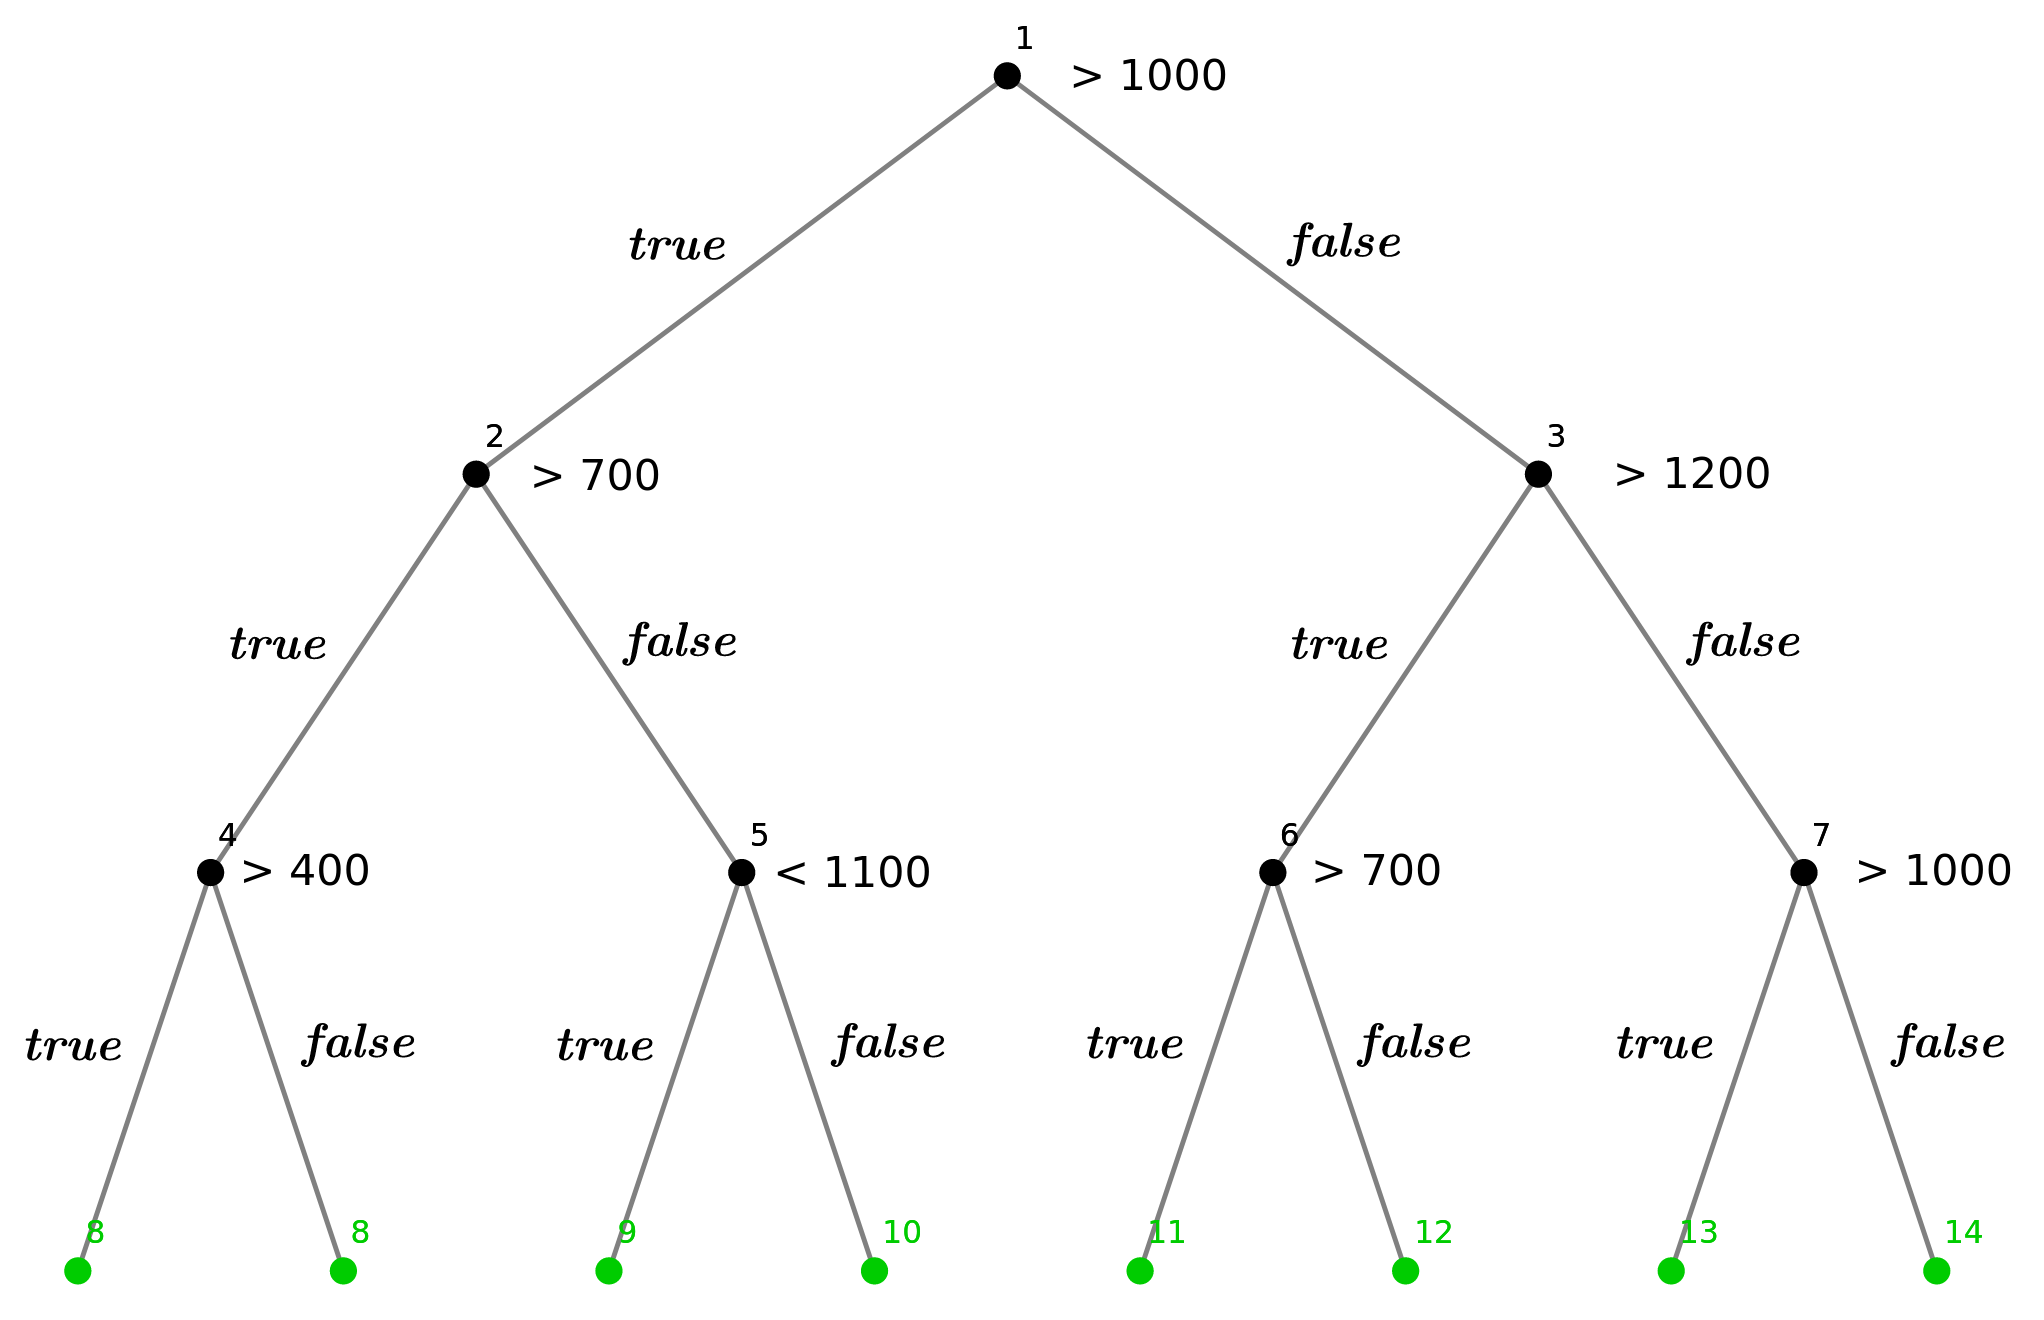
\includegraphics[width=0.69\linewidth]{stablo_primer_1.png}
    \caption{Stablo stanja simboličkog izvršavanja koje odgovara primeru 2. Zelenom bojom su označena završna stanja.}
    \label{fig:moj_primer}
\end{figure}

\begin{minipage}{\linewidth}
\begin{lstlisting}[caption={Primer simboličkog izvršavanja u alatu KLEE},captionpos=b,label={lst:primer_KLEE}]
  void foo(int a) {
    if (a > 1000) {
      a /= 2;
      if (a > 700) {
        a /= 2;
        if (a > 400) {
          a /= 2;
        }
        else {
          return ;
        }
      }
      else {
        a *= 2;
        if (a < 1100) {
          return ;
        }
        else {
          a *= 2;
        }
      }
    }
    else {
      a *= 2;
      if (a > 1200) {
        a /= 2;

        if (a > 700) {
          a /= 2;
        }
        else {
          return ;
        }
      }
      else {
        a *= 2;

        if (a > 1000) {
          a *= 2;
        }
        else {
          a *= 2;
        }
      }
    }
  }
\end{lstlisting}
\end{minipage}
\newpage

\begin{figure}[ht]
    \centering
    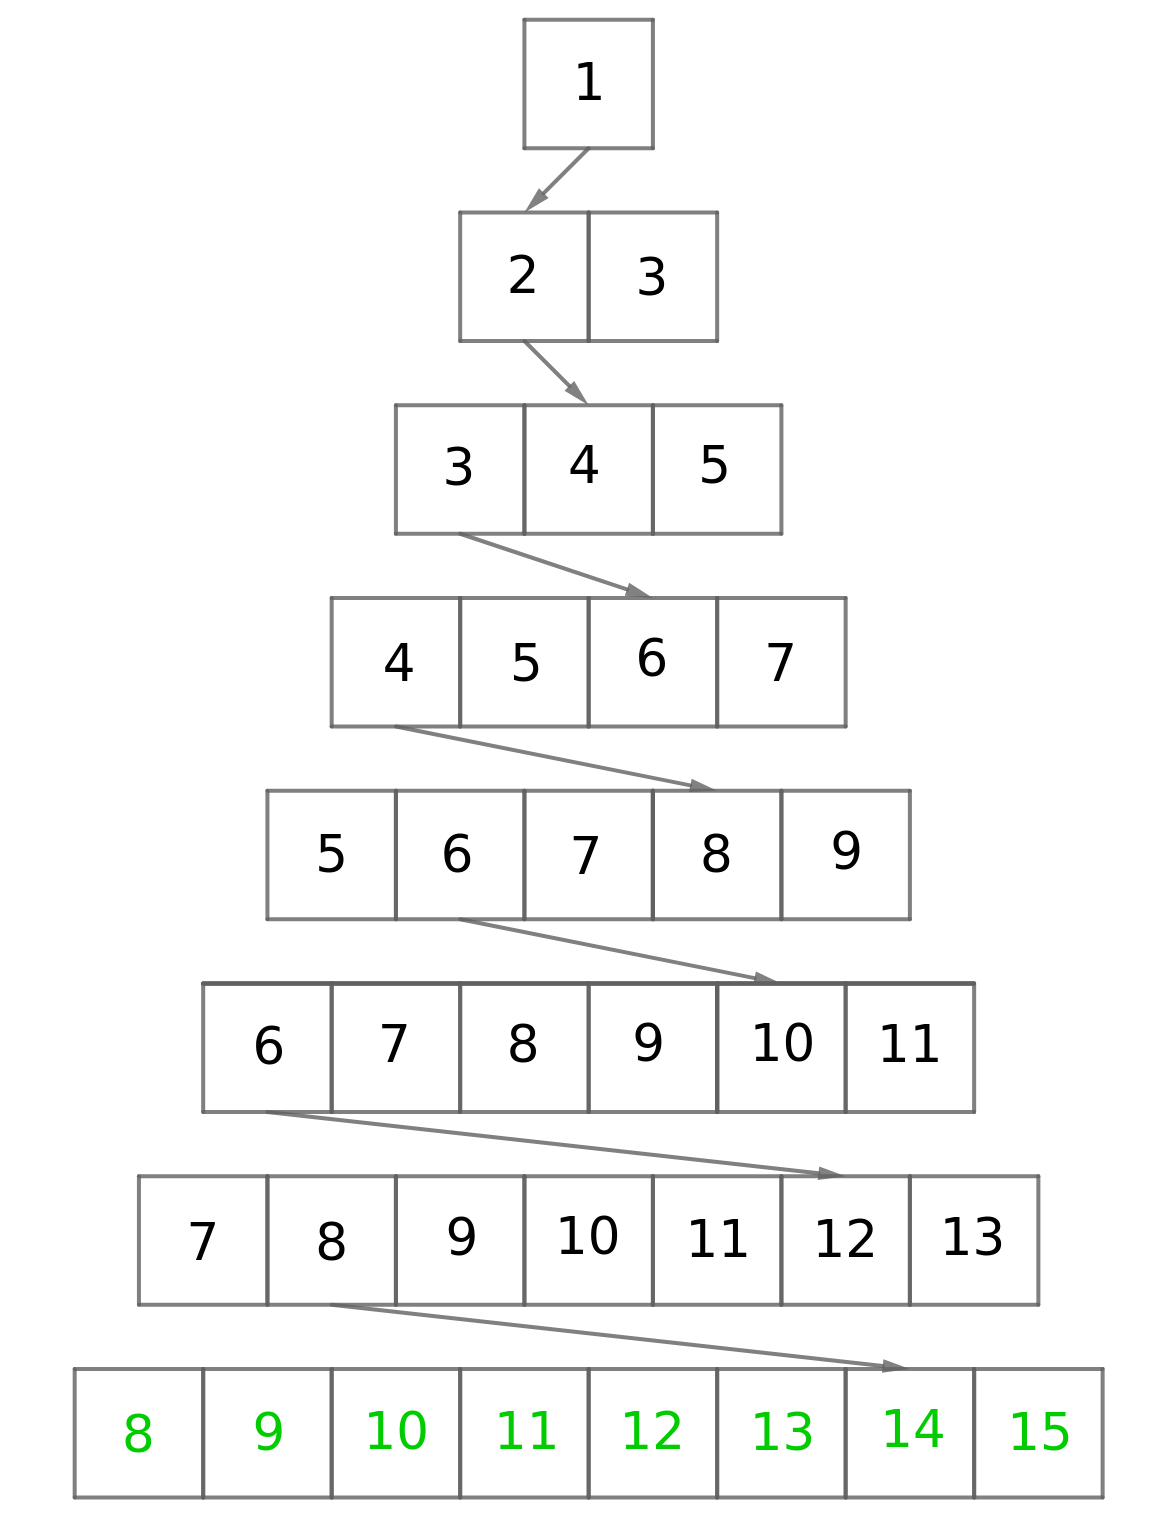
\includegraphics[width=0.75\linewidth]{BFS_stanja_1.png}
    \caption{Pregled izgleda vektora stanja tokom izvršavanja DFS algoritma. Zelenom bojom su prikazana završna stanja, a strelice predstavljaju ''evoluciju'' stanja.}
    \label{fig:BFS_stanja}
\end{figure}
\bigbreak
\textbf{BFS} - Ako pogledamo kako se menja red koji čuva stanja koja se izvršavaju vidimo da se kreće iz stanja 1. Zatim stanje 1 ''evoluira'' u stanje 2 i na kraj reda se dodaje stanje 3. Sledeće stanje koje se uzima je upravo 2, koje dalje ''evoluira'' u stanje 4. Takođe se dodaje novo stanje 5. Stanje 3 mora da ostane na početku reda kako bi bilo naredno izvršeno jer je u pitanju algoritam BFS i potrebno je prvo izvršiti sva stanja na jedno nivou stabla, pa tek onda preći na naredni. Od stanja 3 dobijamo 6 i 7 koji idu na kraj reda. Sledeće stanje koje se izvršava je 4, od koga nastaju 8 i 9. Postupak se nastavlja na prikazani način sve dok u redu ne ostanu samo završna stanja (8 - 15). U tom trenutku će se sva završna stanja izvršiti redom i biti izbacivana iz reda u redosledu izvršavanja. Pošto iz završnog stanja nema gde da se ode dalje, ono se samo izbacuje, time se putanja završava i prelazi se na naredno stanje koje treba izvršiti. 

\begin{figure}[ht]
    \centering
    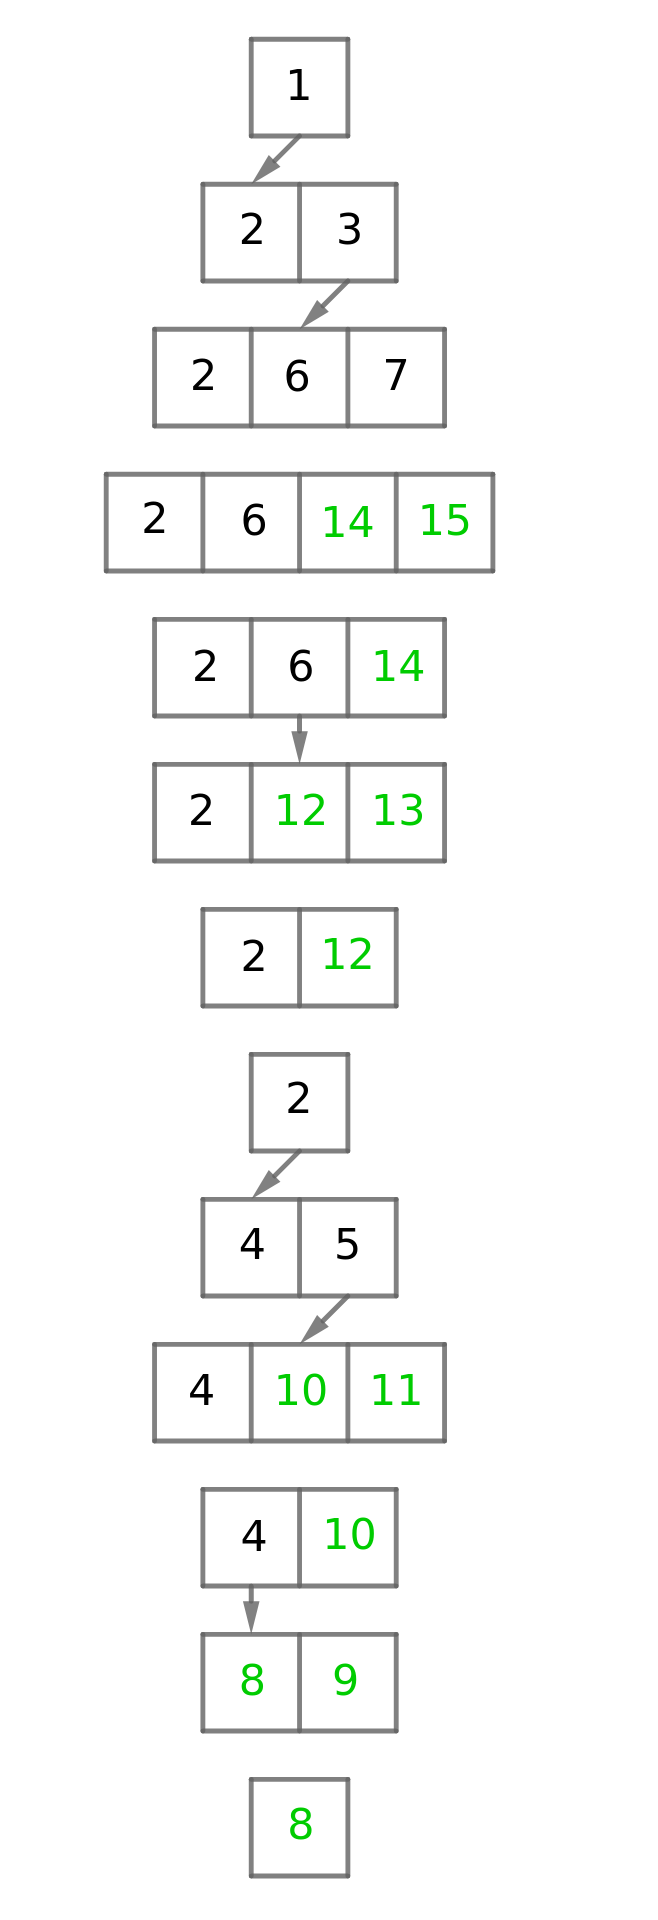
\includegraphics[height=0.8\linewidth]{DFS_states_1.png}
    \caption{Pregled izgleda reda stanja tokom izvršavanja BFS algoritma. Zelenom bojom su prikazana završna stanja, a strelice predstavljaju ''evoluciju'' stanja.}
    \label{fig:DFS_stanja}
\end{figure}
\textbf{DFS} - kod izvršavanja algortima pretrage grafa u dubinu niz stanja se menja na drugačiji način u odnosu na pretragu grafa u širinu. U pitanju je drugačija priroda algoritma. Kod DFS-a se jedna putanja izučava do kraja pa se onda pretraga vraća na grananje gde se bira drugi put. Kod BFS-a se paralelno izučavaju sve putanje. Vidimo da se na početku kreće iz stanja 1 koje evoluira u stanje 2 i dodaje se novo stanje 3 na kraj vektora. Međutim onda se bira baš stanje 3, kao poslednje u vektoru kako bi se simulirala pretraga grafa u dubinu. Nakon toga stanje 3 evoluira u stanje 6 i dodaje se novo stanje 7, dok stanje 2 ostaje i dalje u vektoru ali na početku. Pretraga se nastavlja iz stanja 7 koje evoluira u stanje 14 i dodaje se stanje 15. Kako je sledeće stanje koje se izvršava broj 15, a ono je ujedno i završno stanje, samo se izbacuje iz vektora i prelazi se na stanje 14. Ono je takođe završno pa se pretraga vraća na stanje 6, čime se zapravo izvršio povratak na prethodno grananje (kod stanja 3 na slici). Iz stanja 6 se dobijaju 2 završna stanja, koja nakon izvršavanja bivaju izbačena iz vektora gde ostaje samo stanje 2. Primećujemo da je cela desna polovina stabla stanja izvršena, tj. istražene su sve putanje, pa se pretraga dalje na isti način fokusira na levu plovinu stabla. Iako je u pitanju DFS algoritam koji jednu putanju izvršava do kraja pre nego što pređe na narednu, primećujemo da se sve vreme čuvaju i stanja koja su vezana za putanje koje se ne izučavaju u tom trenutku. Razlog za to je taj što je KLEE \textit{online} alat, kao što je već rečeno u poglavlju \ref{alati_za_simbolicko}.
% ------------------------------------------------------------------------------

% ------------------------------------------------------------------------------
\chapter{Zaključak}
% ------------------------------------------------------------------------------

% ------------------------------------------------------------------------------
% Literatura
% ------------------------------------------------------------------------------
\literatura

% ==============================================================================
% Završni deo teze i prilozi
\backmatter
% ==============================================================================

% ------------------------------------------------------------------------------
% Biografija kandidata
\begin{biografija}
\end{biografija}
% ------------------------------------------------------------------------------

\end{document} 